\documentclass[mat1]{fmfdelo}

\avtor{Aljaž Ostrež}

\naslov{Matrične potence}
\title{Powers of Matrices}

% mentorica, somentor
\mentorica{izr.~prof.~dr.~Marjeta Kramar Fijavž}
\somentor{doc.~dr.~Pavle Boškoski}

\letnica{2021} % leto diplome

%  V povzetku na kratko opišite vsebinske rezultate dela. Sem ne sodi razlaga organizacije dela --
%  v katerem poglavju/razdelku je kaj, pač pa le opis vsebine.
\povzetek{}

%  Prevod slovenskega povzetka v angleščino.
\abstract{}

% navedite vsaj eno klasifikacijsko oznako --
% dostopne so na www.ams.org/mathscinet/msc/msc2020.html
\klasifikacija{}
\kljucnebesede{} % navedite nekaj ključnih pojmov, ki nastopajo v delu
\keywords{} % angleški prevod ključnih besed

\zapisiMetaPodatke  % poskrbi za metapodatke in veljaven PDF/A-1b standard

% aktivirajte pakete, ki jih potrebujete
% \usepackage{tikz}
\usepackage{kbordermatrix}
\usepackage{graphicx}
\usepackage{mathtools}
\usepackage{commath}

% lokacija slik
\graphicspath{{./slike/}}

% za številske množice uporabite naslednje simbole
\newcommand{\R}{\mathbb R}
\newcommand{\N}{\mathbb N}
\newcommand{\Z}{\mathbb Z}
\newcommand{\C}{\mathbb C}
\newcommand{\Q}{\mathbb Q}

% matematične operatorje deklarirajte kot take, da jih bo Latex pravilno stavil
% \DeclareMathOperator{\conv}{conv}

% vstavite svoje definicije ...
%  \newcommand{}{}
\DeclareMathOperator{\Ima}{Im}


\begin{document}

\section{Motivacija}
Z naslednjimi zgledi bomo motivirali uporabo matričnih potenc.
\subsection{Fibonaccijevo zaporedje}

Poglejmo si uporabo matričnih potenc na primeru Fibonaccijevega zaporedja.
\begin{zgled} [Fibonaccijevo zaporedje]
    Poznamo rekurzivno formulo za Fibonaccijevo zaporedje:
    \begin{align*}
        &f_0 = 0, f_1 = 1 \\
        &f_{n+1} = f_n + f_{n-1}, n \geq 1.
    \end{align*}
    Z uvedbo zaporedja $g_n = f_{n-1}$ dobimo sistem:
    \begin{align*}
        f_{n+1} &= f_n + g_n \\
        g_{n+1} &= f_n
    \end{align*}
    ob začetnih pogojih $f_1 = 1$ in $g_1 = 0$. Ta sistem lahko zapišemo v matrični obliki:
    \begin{equation*}
        \begin{bmatrix}
            f_{n+1} \\
            g_{n+1}
        \end{bmatrix}
        =
        \begin{bmatrix}
            1 & 1 \\
            1 & 0
        \end{bmatrix}
        \begin{bmatrix}
            f_n \\
            g_n
        \end{bmatrix}
    \end{equation*}
    za vsak $n \in \mathbb{N}$. Rekurzivno uporabljamo zgornji predpis, da dobimo
    \begin{equation*}
        \begin{bmatrix}
            f_{n+1} \\
            g_{n+1}
        \end{bmatrix}
        =
        \begin{bmatrix}
            1 & 1 \\
            1 & 0
        \end{bmatrix}
        \begin{bmatrix}
            f_n \\
            g_n
        \end{bmatrix}
        =
        \begin{bmatrix}
            1 & 1 \\
            1 & 0
        \end{bmatrix}
        ^2
        \begin{bmatrix}
            f_{n-1} \\
            g_{n-1}
        \end{bmatrix}
        = \cdots =
        \begin{bmatrix}
            1 & 1 \\
            1 & 0
        \end{bmatrix}
        ^n
        \begin{bmatrix}
            f_1 \\
            g_1
        \end{bmatrix}
    \end{equation*}
    oziroma
    \begin{equation*}
        \begin{bmatrix}
            f_{n+1} \\
            g_{n+1}
        \end{bmatrix}
        =
        \begin{bmatrix}
            f_{n+1} \\
            f_n
        \end{bmatrix}
        =
        \begin{bmatrix}
            1 & 1 \\
            1 & 0
        \end{bmatrix}
        ^n
        \begin{bmatrix}
            1 \\
            0
        \end{bmatrix}.
    \end{equation*}
    Z uporabo matričnih potenc torej lahko dobimo ekplicitno formulo za splošni člen v Fibonaccijevemu zaporedju
    \begin{equation*}
        f_n = a_{21},
    \end{equation*}
    kjer je $a_{21}$ prvi element v drugi vrstici matrike:
    \begin{equation*}
        A^n =
        \begin{bmatrix}
            1 & 1 \\
            1 & 0
        \end{bmatrix}
        ^n.
    \end{equation*}
\end{zgled}

Tekom študija smo že spoznali en način za računanje matričnih potenc -- potence matrik lahko računamo s prevedbo na Jordanovo formo.

Naj bo $A \in \mathbb{R}^{m\times m}$ matrika. Potem velja:
\begin{equation*}
    A^n = PJ^nP^{-1},
\end{equation*}
kjer je $J$ Jordanova forma matrike $A$, $P$ pa pripadajoča prehodna matrika. Vemo, da:
\begin{equation*}
    J^n = 
    \begin{bmatrix}
        J_1^n & & \\
         & \ddots & \\
         & & J_k^n
    \end{bmatrix},
\end{equation*}
kjer so $J_i, i=1,\ldots,k$ Jordanovi bloki. Za Jordanove bloke velja:
\begin{equation*}
    J_i^n = 
    \begin{bmatrix}
        \lambda_i^n & {n \choose 1}\lambda_i^{n-1} & \cdots & {n \choose m_i} \lambda_i^{n-m_i} \\
         & \lambda_i^n & \cdots  & {n \choose m_i-1} \lambda_i^{n-(m_i-1)} \\
         & & \ddots  & \vdots \\
         & & & \lambda_i^n
    \end{bmatrix},
\end{equation*}
pri čemer je $\lambda_i$ lastna vrednost matrike $A$, $m_i \times m_i$ pa velikost Jordanovega bloka.
V posebnem primeru, ko je $J$ diagonalna matrika, velja:
\begin{equation*}
    J^n = 
    \begin{bmatrix}
        \lambda_1^n & & \\
         & \ddots & \\
         & & \lambda_m^n
    \end{bmatrix},
\end{equation*}

\begin{zgled} [Fibonaccijevo zaporedje -- nadaljevanje]
    Z izračunom lastnih vrednosti in lastnih vektorjev bi za matriko:
    \begin{equation*}
        A = 
        \begin{bmatrix}
            1 & 1 \\
            1 & 0
        \end{bmatrix}
    \end{equation*}
    dobili Jordanovo formo in prehodno matriko:
    \begin{equation*}
        J = 
        \begin{bmatrix}
                \frac{1+\sqrt{5}}{2} & 0 \\
            0 &  \frac{1-\sqrt{5}}{2}
        \end{bmatrix}
        ,\quad \quad
        P = 
        \begin{bmatrix}
            \frac{1-\sqrt{5}}{2} &  \frac{1+\sqrt{5}}{2} \vspace{2pt} \\
            1 & 1
        \end{bmatrix}.
    \end{equation*}
    Naš sistem enačb lahko zapišemo kot:
    \begin{equation*}
        \begin{bmatrix}
            f_{n+1} \\
            f_n
        \end{bmatrix}
        =
        A^n
        \begin{bmatrix}
            1 \\
            0
        \end{bmatrix}
        = PJ^n P^{-1}
        \begin{bmatrix}
            1 \\
            0
        \end{bmatrix}.
    \end{equation*}
    Izračunamo, da je:
    \begin{equation*}
        f_n = \frac{\sqrt{5}}{5}\Big[ \Big(\frac{1+\sqrt{5}}{2}\Big)^n - \Big(\frac{1-\sqrt{5}}{2}\Big)^n \Big], \quad n \in \mathbb{N}_0.
    \end{equation*}
    S pomočjo matričnih potenc smo dobili eksplicitno formulo zaporedja iz rekurzivnega predpisa.
\end{zgled}

Zakaj potrebujemo nove metode za računanje matričnih potenc, če jih že znamo računati s pomočjo Jordanove forme? Izkaže se, da je izračun Jordanove forme numerično zahteven, poleg tega pa nam Jordanova forma omogoča potenciranje matrik le v končnih dimenzijah. Velikokrat nam tudi ni potrebno izračunati celotne matrike $A^n$, ampak želimo le poznati nekatere njene lastnosti. Namesto Jordanove forme bomo uporabili spektralni razcep, ki ni odvisen od izbire baze matrike $A$.

Želeli bomo opisati asimptotsko obnašanje matričnih zaporedij s splošnim členom $A_n = A^n$, kjer je $A \in \R^{m \times m}$. To obnašanje se lahko razbere že iz spektra matrike, včasih pa celo le iz spektralnega radija.

\subsection{Markovske verige}

Uporabo matričnih potenc bomo prikazali na primeru markovskih verig. Navedimo definicijo markovske verige.
\begin{definicija}
    Naj bo $S$ števna množica, ki jo poimenujemo \emph{množica stanj}. Njene elemente $s \in S$ imenujemo \emph{stanja}. \emph{Slučajni proces} (z diskretnim časom) je vsako zaporedje diskretnih slučajnih spremenljivk $X_0, X_1, \ldots, X_n, \ldots$, katerih zaloga vrednosti leži v $S$. To zaporedje imenujemo \emph{markovska veriga}, če ima markovsko lastnost:
    \begin{equation}
        P(X_n = s_n | X_0 = s_0, X_1 = s_1, \ldots, X_{n-1} = s_{n-1}) = P(X_n = s_n | X_{n-1} = s_{n-1}),
    \end{equation}
    tj. verjetnost stanja na $n$-tem koraku je odvisna le od stanja na $(n-1)$-tem koraku. Vpeljemo še pojma \emph{prehodne verjetnosti} $p_{ij} = P(X_n = s_j | X_{n-1} = s_i)$ in \emph{prehodne matrike} $P = (p_{ij})$.
\end{definicija}
Poglejmo si zgled markovske verige, ki bo hkrati tudi motiviral računanje limite zaporedja $A_n = A^n$, če ta obstaja. 
\begin{zgled}
    Izberimo si vozlišče na poljubnem neusmerjenem grafu. Izberemo si naključnega soseda izbranega vozlišča in se premaknemo v njega. Postopek ponavljamo. Kakšen je delež obiskov določenega vozlišča v grafu po dolgem času? Ker soseda izbiramo naključno, začetnemu grafu priredimo utežen usmerjen graf, kjer so uteži verjetnosti, da se premaknemo v povezanega soseda. Tu privzamemo, da so izbire sosedov enako verjetne, za vozlišče stopnje $k$ so vse verjetnosti enake $\frac{1}{k}$.
    \begin{figure}[!htb]
        \centering
        \begin{minipage}{0.5\textwidth}
            \centering
            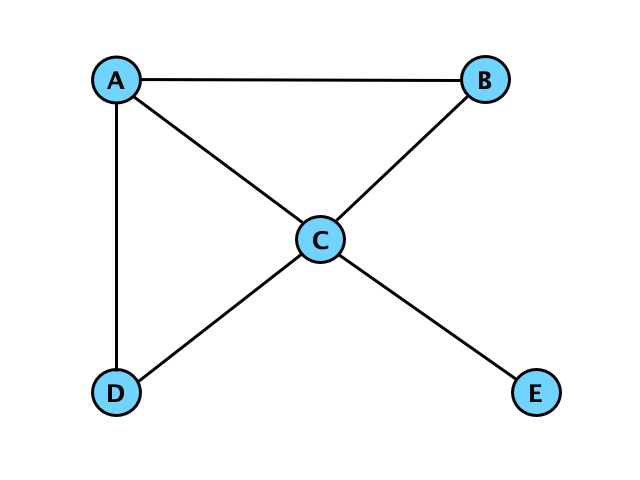
\includegraphics[width=\textwidth]{grafUndir.png}
            \caption{Začetni neusmerjen graf.}
        \end{minipage}
        \hspace{-30pt}
        \begin{minipage}{0.5\textwidth}
            % \vspace{30pt}
            \centering
            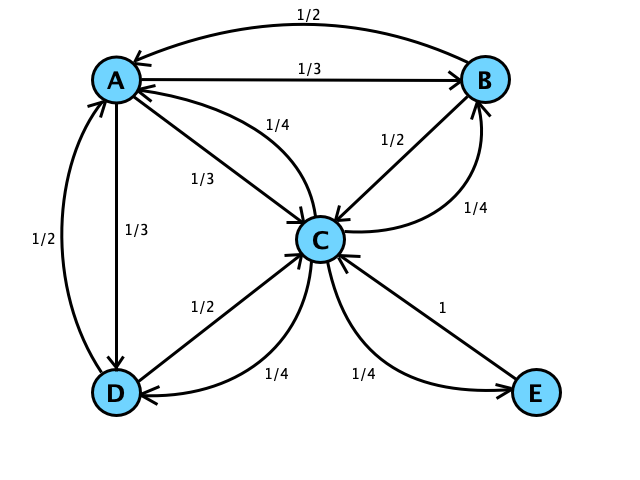
\includegraphics[width=\textwidth]{grafDir.png}
            \caption{Prirejen utežen usmerjen graf.}
        \end{minipage}
    \end{figure}

    \noindent Naša množica stanj je $S = \{A, B, C, D, E\}$, prehodna matrika pa bo kar matrika sosednosti prirejenega uteženega usmerjenega grafa
    \begin{equation*}
        P =
        \kbordermatrix{
                & A & B & C & D & E \\
            A & 0 & 1/3 & 1/3 & 1/3 & 0 \\
            B & 1/2 & 0 & 1/2 & 0 & 0 \\
            C & 1/4 & 1/4 & 0 & 1/4 & 1/4 \\
            D & 1/2 & 0 & 1/2 & 0 & 0 \\
            E & 0 & 0 & 1 & 0 & 0
        }.
    \end{equation*}
    Ker je izbira naslednjega vozlišče v zaporedju odvisna le od trenutnega vozlišča, ima naše zaporedje markovsko lastnost, torej bo naša pot v grafu markovska veriga. Kaj nam pa pove prehodna matrika?
    \begin{itemize}
        \item Matrika $P$ nam pove, kakšna je verjetnost, da bomo prišli v določeno vozlišče v naslednjem koraku, če smo trenutno v vozlišču, ki ga predstavlja vrstica.
        \item $P^2$ nam pove, kakšna je verjetnost, da bomo prišli v določeno vozlišče čez 2 koraka.
        \item ...
    \end{itemize}
    Za naš primer se izkaže celo, da obstaja limita:
    \begin{equation*}
        \lim_{n \rightarrow \infty} P^n =
        \begin{bmatrix}
            0,25 & 0,17 & 0,33 & 0,17 & 0,08 \\
            0,25 & 0,17 & 0,33 & 0,17 & 0,08 \\
            0,25 & 0,17 & 0,33 & 0,17 & 0,08 \\
            0,25 & 0,17 & 0,33 & 0,17 & 0,08 \\
            0,25 & 0,17 & 0,33 & 0,17 & 0,08 
        \end{bmatrix}.
    \end{equation*}
    Ta limita nam pove delež obiskov za vsako vozlišče (če bi zelo dolgo potovali). Limita je tudi neodvisna od izbire začetnega vozlišča, če je le graf povezan.
\end{zgled}

\subsection{Ponovitev iz linearne algebre}\label{linearnaAlgebra}
Naj bo $A \in \C^{n \times n}$ matrika dimenzije $n \times n$. Definiramo \emph{množico polinomov matrike} $A$ s predpisom
\begin{equation}
    \mathcal{P}_A := \Big\{ \sum_{i=0}^m \alpha_i A^i\ |\  \alpha_i \in \C, m \in \N_0 \Big\} \subset \C^{n \times n}.
\end{equation}
Če je $p(x) = \sum_{i=0}^m \alpha_i x^i$ polinom, bomo pisali
\begin{equation}
    p(A) := \sum_{i=0}^m \alpha_i A^i.
\end{equation}
Definiramo preslikavo
\begin{align}
\begin{split}
    \Phi_A : \C [x] &\longrightarrow \mathcal{P_A} \\
    p &\longmapsto p(A),
\end{split}
\end{align}
kjer je $\C [x]$ množica polinomov s koeficienti iz $\C$. Jedro preslikave $\Phi_A$ je
\begin{equation}
    \ker (\Phi_A) = \Big\{ p \in \C [x] \ | \  p(A) = 0 \Big\},
\end{equation}
torej $\ker(\Phi_A)$ je množica vseh polinomov, za katere je $p(A) = 0$.

\begin{definicija}
    \emph{Minimalni polinom} $m_A \in \C[x]$ je neničeln monični polinom najmanjše stopnje iz $\ker(\Phi_A)$, tj.\ monični polinom najnižje stopnje, za katerega je $P(A) = 0$.
\end{definicija}
\begin{opomba}
    \emph{Monični polinom} je polinom z vodilnim koeficientom enakim 1.
\end{opomba}
Spomnimo se, da je minimalni polinom $m_A$ enolično določen z matriko $A$. Potrebovali bomo še pojem \emph{lastne vrednosti} in \emph{lastnega vektorja} matrike $A$, osvežimo pa še definicijo \emph{karakterističnega polinoma} matrike $A$. Poleg tega navedimo še definicijo \emph{lastnega podprostora}.
\begin{definicija}
    Naj bo $A \in \C^{n \times n}$.
    \begin{itemize}
        \item Število $\lambda \in \C$ imenujemo \emph{lastna vrednost} matrike $A$, če obstaja vektor $x \in \C^n$, tako da velja
        \begin{equation}
            Ax = \lambda x.
        \end{equation}
        Vektorji $x$, za katere velja zgornja enačba, so pripadajoči \emph{lastni vektorji}.
        \item Polinom
        \begin{equation}
            \Delta_A(\lambda) = \det (A - \lambda I) \in \mathcal{P}_A
        \end{equation}
        v spremenljivki $\lambda$ imenujemo \emph{karakteristični polinom} matrike $A$.
        \item \emph{Lastni podprostor} matrike $A$, ki pripada lastni vrednosti $\lambda$, je definiran kot $\ker (A - \lambda I)$.
    \end{itemize}
\end{definicija}
\emph{Algebraična večkratnost} lastne vrednosti $\lambda$ je večkratnost $\lambda$ kot ničle polinoma $\Delta_A(\lambda)$. \emph{Geometrična večkratnost} lastne vrednosti $\lambda$ pa je dimenzija pripadajočega lastnega podprostora $\ker (A - \lambda I)$.
Brez dokaza se spomnimo naslednje trditve, s pomočjo katere med drugim tudi na roke iščemo lastne vrednosti matrike $A$.
\begin{trditev}
    Naj bo $A \in \C^{n \times n}$, $m_A$ pripadajoči minimalni polinom, $\Delta_A$ pripadajoči karakteristični polinom in $\lambda \in \C$. Naslednje trditve so ekvivalentne:
    \begin{enumerate}
        \item $\lambda$ je lastna vrednost matrike $A$,
        \item $\lambda$ je ničla polinoma $m_A$,
        \item $\lambda$ je ničla polinoma $\Delta_A$.
    \end{enumerate}
\end{trditev}
Iz zgornje trditve sledi, da lahko minimalni polinom $m_A$ matrike $A$ zapišemo kot
\begin{equation}
    m_A(z) = (z-\lambda_1)^{\nu_1}(z-\lambda_2)^{\nu_2}\cdots (z-\lambda_m)^{\nu_m},
\end{equation}
kjer $\lambda_1, \ldots, \lambda_m$ lastne vrednosti matrike $A$, $\nu_1, \ldots, \nu_m$ pa pripadajoče \textbf{???geometrične???} večkratnosti.

V nadaljevanju bomo omenjali tudi \emph{matrične} in \emph{operatorske norme}.
\begin{definicija}
    \emph{Matrična norma} je preslikava $\norm{\cdot}: \C^{n \times n} \longrightarrow \R$. Za vsaki matriki $A, B \in \C^{n \times n}$ in vsak skalar $\alpha \in \C$ velja:
    \begin{enumerate}
        \item $\norm{A} \geq 0$ in $\norm{A} = 0$ natanko tedaj, ko je $A = 0$ (pozitivnost),
        \item $\norm{\alpha A} = |\alpha|\norm{A}$ (homogenost),
        \item $\norm{A + B} \leq \norm{A} + \norm{B}$ (trikotniška neenakost), 
        \item $\norm{A B} \leq \norm{A} \norm{B}$ (submultiplikativnost). Matrične norme, ki so porojene iz vektorskih norm s predpisom
        \begin{equation}
            \norm{A} = \max_{x \neq 0} \frac{\norm{A x}}{\norm{x}},
        \end{equation}
        imenujemo operatorske norme.
    \end{enumerate} 
\end{definicija}

\section{Spektralni razcep}
\subsection{Matrični polinomi}
$R$
V podpoglavju \ref{linearnaAlgebra} smo že definirali množico matričnih polinomov $\mathcal{P}_A$ in minimalni polinom $m_A$ matrike $A \in \C^{n \times n}$, pa tudi preslikavo $\Phi_A$ iz množice polinomov $\C [x]$ v $\mathcal{P}_A$.
\begin{trditev}\label{trditevMinimalniPolinom}
    Naj bo $m_A$ minimalni polinom. Potem je
    \begin{equation}
        p \in \ker (\Phi_A) \Leftrightarrow p = m_A \cdot q\ \  \text{za}\ \ q \in \C [x],
    \end{equation}
    tj.\ $p(A) = 0$ natanko tedaj, ko je $p(A)$ večkratnik minimalnega polinoma $m_A$.
\end{trditev}
\begin{dokaz}
    Najprej dokažimo implikacijo ($\Leftarrow$). Naj bo $m_A$ minimalni polinom. Če je $p = m_A\cdot q$ za nek $q \in \C [x]$, potem je
    \begin{equation}
        p(A) = m_A(A) \cdot q(A) = 0 \cdot q(A) = 0,
    \end{equation}
    torej je $p \in \ker(\Phi_A)$.
    
    \noindent Dokažimo še ($\Rightarrow$). Naj bo $p \in \C [x]$, za katerega velja $p(A) = 0$. Če delimo $p$ z $m_A$, dobimo:
    \begin{equation*}
        p = m_A \cdot q + r
    \end{equation*}
    za $q, r \in \C [x]$, da velja $\text{st}(r) < \text{st}(q)$. Velja
    \begin{equation*}
        0 = p(A) = \underbrace{m_A(A)}_{=0} \cdot q(A) + r(A) = r(A),
    \end{equation*}
    torej je $r \in \ker(\Phi_A)$. Ker ima $m_A$ najmanjšo stopnjo v $\ker(\Phi_A)$, sklepamo, da je $r \equiv 0$.
\end{dokaz}
Za polinome $p, q, r \in \C [x]$ bomo uporabljali zapis
\begin{equation}
    p \equiv q \mod r\  \Longleftrightarrow\  p - q = s\cdot r\ \  \text{za nek}\  s\in \C [x].
\end{equation}

Poglejmo si posledico trditve \ref{trditevMinimalniPolinom}
\begin{posledica} \label{posledicaProjekcija}
    Naj bosta $p, q \in \C [x]$. Velja
    \begin{equation}
        p(A) = q(A)\  \Longleftrightarrow\ p \equiv q \mod m_A.
    \end{equation}
    V posebnem primeru velja, da je $p(A)$ projekcija natanko tedaj, ko je $p^2 \equiv p \mod m_A$.
\end{posledica}
\begin{trditev} \label{trditevPosploseniMinimalni}
    Naj bosta $p, q \in \C [x]$. Za vsak $i = 1, \ldots, m$ in $\nu = 0, \ldots, \nu_i-1$ velja
    \begin{equation}
        p \equiv q \mod m_A \ \Longleftrightarrow\  p^{(\nu)}(\lambda_i) = q^{(\nu)}(\lambda_i).
    \end{equation}
\end{trditev}
\begin{dokaz}
    Trditev sledi iz dejstva, da za nek $n\in \N$ in neničeln $q \in \C [x]$ ter fiksen $z_1 \in \C$ velja
    \begin{equation*}
        p(z) = (z-z_1)^n q(z) \ \Longleftrightarrow\  p^{(i)}(z_1)=0 \ \text{za}\  i=0, 1, \ldots, n-1,
    \end{equation*}
    kar smo že dokazali pri študiju algebre.
\end{dokaz}

\subsection{Gladke matrične funkcije}

Naj bo $A \in \C^{n \times n}$ matrika z minimalnim polinomom $m_A$. Naj bodo $\lambda_1, \ldots, \lambda_m$ ničle $m_A$ z večkratnostimi $\nu_1, \ldots, \nu_m$. Definirajmo množico funkcij, ki so definirane in neskončnokrat odvedljive na okolici $\{\lambda_1, \ldots, \lambda_m\}$, s predpisom
\begin{equation}
    C_A^\infty := \{ f: D(f) \rightarrow \C\ |\ \exists U \subset D(f)\ \text{odprta}, \{\lambda_1, \ldots, \lambda_m\} \subset U, f|_U \in C^\infty \},
\end{equation}
kjer je $D(f) \subset \C$ definicijsko območje funkcije $f$.
\begin{definicija} \label{definicijaGladkaFunkcija}
    Naj bo $f \in \C_A^\infty$. Definiramo:
    \begin{equation}
        f(A) := \Phi_A(p_f) = p_f(A),
    \end{equation}
    kjer je $p_f$ polinomska interpolacija funkcije $f$, ki zadošča pogoju
    \begin{equation}
        f^{(\nu)}(\lambda_i) = p_f^{(\nu)}(\lambda_i)
    \end{equation}
    za vsak $i = 1, \ldots, m$ in $\nu = 0, \ldots, \nu_i-1$.
\end{definicija}
S to definicijo lahko matrične polinome razširimo na množico gladkih matričnih funkcij:
\begin{align}
    \begin{split}
        \widetilde{\Phi} :\ &C_A^\infty \longrightarrow \mathcal{P_A} \\
        &\widetilde{\Phi}_A(f) = \Phi_A(p_f) = p_f(A)
    \end{split}
\end{align}
Iz definicije \ref{definicijaGladkaFunkcija} in trditev \ref{trditevMinimalniPolinom}, \ref{trditevPosploseniMinimalni} sledi:
\begin{trditev} \label{trditevPhiAlgebra}
    Naj bodo oznake kot zgoraj. Velja:
    \begin{enumerate}
        \item Definicija $\widetilde{\Phi}_A(f)$ ni odvisna od izbire metode za polinomsko interpolacijo $p_f$.
        \item Preslikava $\widetilde{\Phi}_A$ je razširitev funkcije $\Phi_A$.
        \item $\widetilde{\Phi}$ je homomorfizem algeber, kar pomeni, da velja:
        \begin{align*}
            \widetilde{\Phi}_A(\lambda f + \mu g) &= \lambda \widetilde{\Phi}_A(f) + \mu \widetilde{\Phi}_A(g), \\
            \widetilde{\Phi}_A(f \cdot g) &= \widetilde{\Phi}_A(f) \cdot \widetilde{\Phi}_A(g)
        \end{align*}
        za $\lambda, \nu \in \C$ in $f, g \in C_A^\infty$.
    \end{enumerate}
\end{trditev}

Definirajmo \emph{karakteristično funkcijo} $\chi_U$ s predpisom
\begin{equation}
    \chi_U(\lambda) =
    \begin{cases}
        1, \lambda \in U, \\
        0, \lambda \notin U
    \end{cases}
\end{equation}
za odprte množice $U \subset \C$, za katere velja $\{\lambda_1, \ldots, \lambda_m\} \in U$. Funkcija $\chi_U$ je idempotent, kar pomeni, da velja $\chi_U \cdot \chi_U = \chi_U$. Po posledici \ref{posledicaProjekcija} sklepamo, da je $\chi_U(A) \in \mathcal{P}_A$ projekcija, ki komutira z A. Vzemimo posebno množico takšnih projekcij.
\begin{definicija}
Naj bodo $U_1, \ldots, U_m \subset \C$ odprte množice, ki zadostujejo pogojema:
\begin{enumerate}
    \item $\lambda_i \in U_i$ za $i = 1,\ldots,m$ in
    \item $U_i \cap U_j = \emptyset$ za $i \neq j$.
\end{enumerate}
Z $\chi_i$ označimo karakteristično funkcijo množice $U_i$. Polinomi
\begin{equation} \label{definicijaProjekcije}
    P_i := \chi_i(A) \in \mathcal{P}_A\ \text{za}\ i = 1,\ldots, m,
\end{equation}
so {spektralne projekcije}, njihovo zalogo vrednosti pa bomo označili z 
\begin{equation} \label{zalogeProjekcij}
    X_i := \Ima P_i.
\end{equation}
\end{definicija}
Omenimo, da je $P_i$ neodvisna od izbire $U_i$, poleg tega pa velja še $P_i \neq 0$ za vsak $i$.

\begin{trditev}
    Naj $A \in \C^{n \times n}$ matrika z minimalnim polinomom $m_A$, z ničlami $\lambda_1, \ldots, \lambda_m$ in z večkratnostmi $\nu_1, \ldots, \nu_m$. Če vzamemo $P_i$ in $X_i$ kot v \eqref{definicijaProjekcije} in \eqref{zalogeProjekcij}, potem je
    \begin{equation}
        X = X_1 \oplus \cdots \oplus X_m
    \end{equation}
    razcep direktnih vsot v A-invariantne podprostore z omejitvijo, da je $A - \lambda_i I$ nilpotentna reda $\nu_i$ na $X_i$ za $i = 1, \ldots, m$.
\end{trditev}
\begin{dokaz}
    Ker so množice $U_i$ disjunktne, velja $\chi_i(\sum_{i \neq j} \chi_j) = 0$, torej tudi $P_i(\sum_{i \neq j} P_j) = 0$. Iz tega sledi, da je
    \begin{equation}
        X_i \hat (\bigoplus_{i \neq j} X_j) = {}
    \end{equation}
\end{dokaz}

\begin{trditev} \label{trditevFormula}
    Naj bo $A \in \mathcal{L}$ z lastnimi vrednostmi $\lambda_1, \lambda_2, \ldots, \lambda_m$, ki imajo po vrsti večkratnosti $\nu_1, \nu_2, \ldots, \nu_m$. Definirajmo projekcije $P_i$ kot v \eqref{definicijaProjekcije}. Tedaj za vsako funkcijo $f \in C_A^\infty$ velja
    \begin{equation}
        f(A) = \sum_{i=1}^m \sum_{\nu = 0}^{\nu_i - 1} \frac{f^{(\nu)}(\lambda_i)}{\nu !}(A - \lambda_i)^\nu P_i.
    \end{equation}
\end{trditev}
\begin{dokaz}
    Funkcija
    \begin{equation}
        g(\lambda) = \sum_{i=1}^m \sum_{\nu = 0}^{\nu_i - 1} \frac{f^{(\nu)}(\lambda_i)}{\nu !}(\lambda - \lambda_i)^\nu \chi_i(\lambda), \quad \lambda \in \C,
    \end{equation}
    sovpada z $f$, vključno z vsemi pomembnimi odvodi, na vseh točkah $\lambda_1, \ldots, \lambda_m$.  Po trditvah \ref{trditevPosploseniMinimalni} in \ref{trditevPhiAlgebra} sledi, da je $f(A) = g(A)$.
\end{dokaz}
\begin{posledica}
    Naj bodo predpostavke enake kot v trditvi \ref{trditevFormula}. Za $k \in \N$ velja
    \begin{equation}
        A^k = \sum_{i=1}^m \sum_{\nu = 0}^{\min \{\nu_i - 1, k\}} {k \choose \nu} \lambda_i^{k-\nu}(A - \lambda_i)^\nu P_i.
    \end{equation}
\end{posledica}
\begin{dokaz}
    V trditvi \ref{trditevFormula} za $k \in \N$ uporabimo funkcijo $f(\lambda) = \lambda^k$.
\end{dokaz}

\subsection{Spektralna teorija}


\begin{definicija}
Projekciji $P_i$, definirani kot v \eqref{definicijaProjekcije}, rečemo \emph{spektralna projekcija}, prostoru $X_i := P_i X$ pa \emph{spektralni podprostor} lastne vrednosti $\lambda_i$. Množici $\sigma(A) := \{\lambda_1, \ldots, \lambda_m\}$ rečemo \emph{spekter} matrike A.
\end{definicija}

Navedimo še definicijo zelo uporabne lastnosti spektra.

\begin{definicija}
    Naj bo $T \in \mathcal{L}(X)$ in $\sigma(T)$ spekter operatorja $T$. \emph{Spektralni radij} definiramo kot
    \begin{equation}
        r(T) := \max \{|\lambda|, \lambda \in \sigma(T)\},
    \end{equation}
    tj. absolutno največja lastna vrednost operatorja $T$.
\end{definicija}

\begin{izrek} [Izrek o preslikavi spektra]\label{izrekOPreslikaviSpektra}
    Naj bo $A \in \mathcal{L}(X)$ in $f \in C_A^\infty$. Potem velja
    \begin{equation}
        \sigma\big(f(A)\big) = f\big(\sigma(A)\big) := \{f(\lambda) | \lambda \in \sigma(A)\}.
    \end{equation}
\end{izrek}

\begin{lema}\label{lemaNorme}
    Naj bo $\norm{\cdot}$ norma na $\C^{n \times n}$. Za $A \in \C^{n \times n}$ in $\mu > r(T)$ obstajata konstanti $N > 0$ in $M > 1$, da za vse $k \in \N$ velja
    \begin{equation}
        N \cdot r(T) \leq \norm{T^k} \leq M \cdot \mu^k.
    \end{equation}
    Če je $\norm{\cdot}$ operatorska norma, izberemo $N = 1$.
\end{lema}

\begin{trditev} [Gelfandova formula]
    Za matriko $A \in \C^{n \times n}$ velja:
    \begin{enumerate}
        \item $r(T) = \lim_{k \rightarrow \infty} \norm{T^k}^{1/k}$ za vsako matrično normo $\norm{\cdot}$ na $\C^{n \times n}$,
        \item če je $\norm{\cdot}$ operatorska norma na $C^{n \times n}$, potem je $r(T) = \inf_{k > 0} \norm{T^k}^{1/k}$.
    \end{enumerate}
\end{trditev}

\begin{dokaz}
    Uporabimo posledico leme \ref{lemaNorme}
    \begin{equation*}
        N^{1/k} r(T) \leq \norm{T^k}^{1/k} \leq M^{1/k} \mu.
    \end{equation*}
    To smo dobili tako, da smo enačbo v lemi pomnožili z $\frac{1}{k}$. Če je $\norm{\cdot}$ operatorska norma, za dopustno izbiro $N = 1$ dobimo $r(T) = \inf_{k > 0} \norm{T^k}^{1/k}$.
\end{dokaz}


\section{Zaporedja matričnih potenc}
\subsection{Koordinatna zaporedja}

\subsection{Asimptotsko obnašanje}
\begin{definicija}
    Naj bo $T \in \mathcal{L}(X)$ in $\norm{\cdot}$ neka matrična norma. Zaporedje $(T^k)$ je:
    \begin{itemize}
        \item omejeno, če je $\sup_{k \in \N} \norm{T^k} < \infty$;
        \item stabilno, če je $\lim_{k \rightarrow \infty} \norm{T^k} = 0$;
        \item konvergentno, če je $\lim_{k \rightarrow \infty} T^k = P$ za nek $P \in \mathcal{L}(X)$;
        \item periodično s periodo $p$, če je $T^p = I$;
        \item Ces\`aro sumabilno, če obstaja limita $\lim_{k \rightarrow \infty} \Big(\frac{1}{k}\sum_{l=0}^{k-1} T^l\Big)$.
    \end{itemize}
\end{definicija}

\section{Primer uporabe}

\section*{Slovar strokovnih izrazov}

\geslo{}{}
\geslo{}{}

% seznam uporabljene literature
\begin{thebibliography}{99}

\bibitem{agbinya} J.~I.~Agbinya, \emph{Applied Data Analytics -- Principles and Applications}, River Publishers, Denmark, 2020.

\bibitem{kramar} A.~B\'{a}tkai, M.~Kramar Fijavž in A.~Rhandi, \emph{Positive Operator Semigroups From Finite To Infinite Dimensions}, Birkh\"{a}user/Springer, 2017.

\bibitem{meyer} C.~Meyer, \emph{Matrix Analysis and Applied Linear Algebra}, SIAM, 2000.


\end{thebibliography}

\end{document}

